\chapter{Выполнение работы}

\section{Задания по исходной программе}

\subsection{Листинги исходной программы}

Исходный текст программы test.s приведен в листинге~\ref{lst:test:src}

\lstinputlisting[label=lst:test:src,caption=Исходный код программы text.s, captionpos=b]{listings/test.s}
\clearpage

Листинг программы test, полученный через makefile, приведен в листинге~\ref{lst:test:lst}

\lstinputlisting[label=lst:test:lst,caption=Листинг программы test полученный через makefile, captionpos=b]{listings/test.lst}

16-ричный набор команд программы test приведен в листинге~\ref{lst:test:hex}

\lstinputlisting[label=lst:test:hex,caption=Команды программы test в 16-ричном формате, captionpos=b]{listings/test.hex}

Псевдокод поясняющий работу программы test приведен в листинге~\ref{lst:test:pseudo}

\lstinputlisting[label=lst:test:pseudo,caption=Псевдокод к программе test, captionpos=b]{pseudo/pseudo_test.txt}
\clearpage

\subsection{Скриншоты к исходной программе}

Стадии выборки и диспетчеризации (fetch\&dispatch, или F+ID) 1-й итерации команды 80000014 (согласно варианту) приведена на рисунке~\ref{img:task2}

\begin{figure}[H]
	\centering
	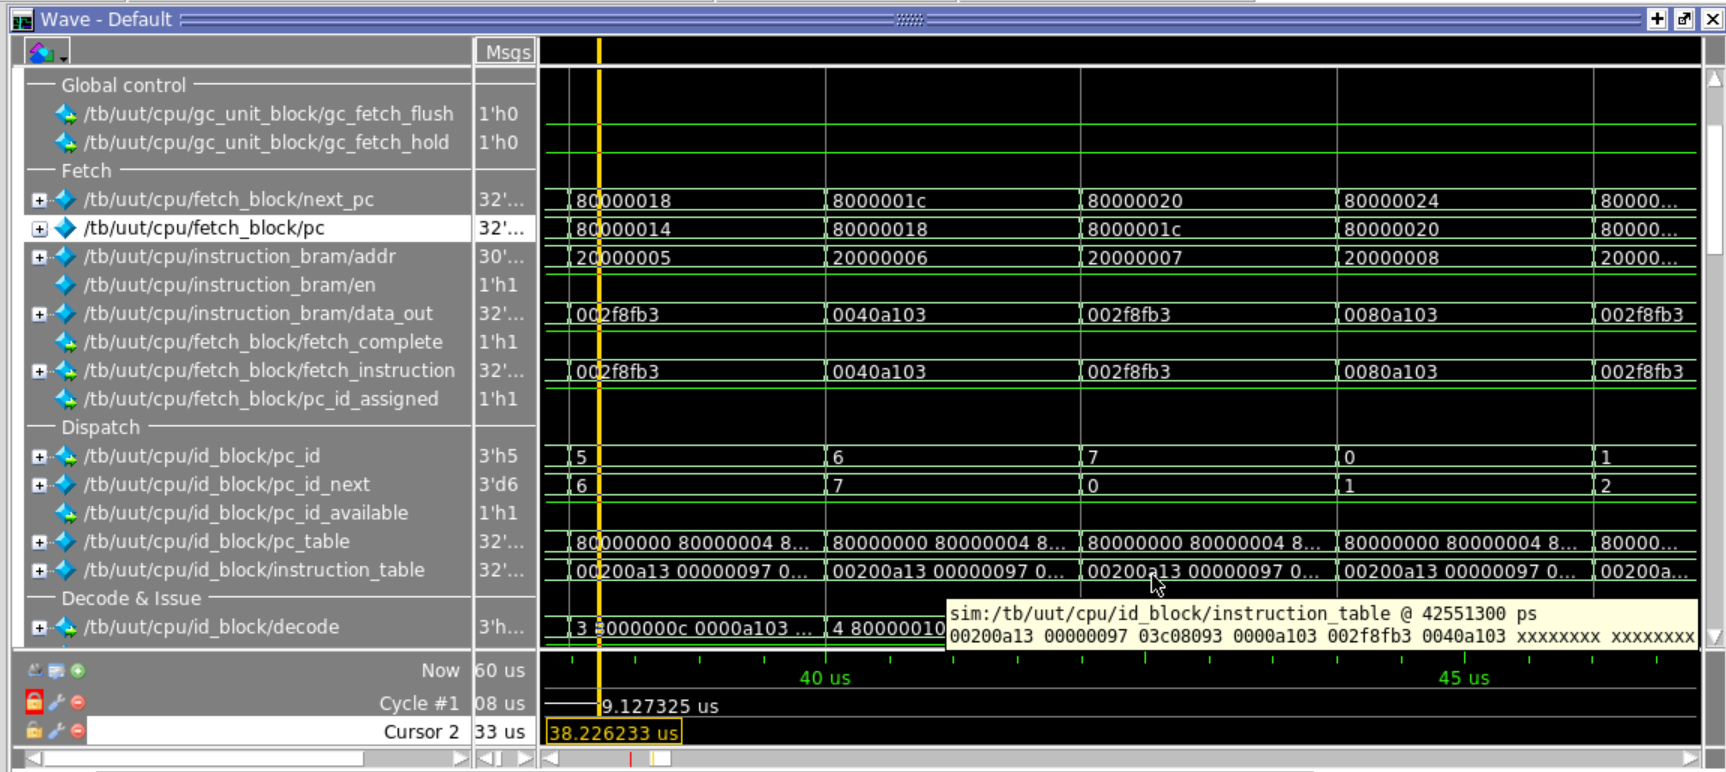
\includegraphics[width=1\textwidth]{images/task2.png}
	\caption{Стадии выборки и диспетчеризации 1-й итерации команды 80000014}
	\label{img:task2}
\end{figure}

Стадия декодирования и планирования (decode\_and\_issue, или D) 1-й итерации команды 80000020 (согласно варианту) приведена на рисунке~\ref{img:task3}

\begin{figure}[H]
	\centering
	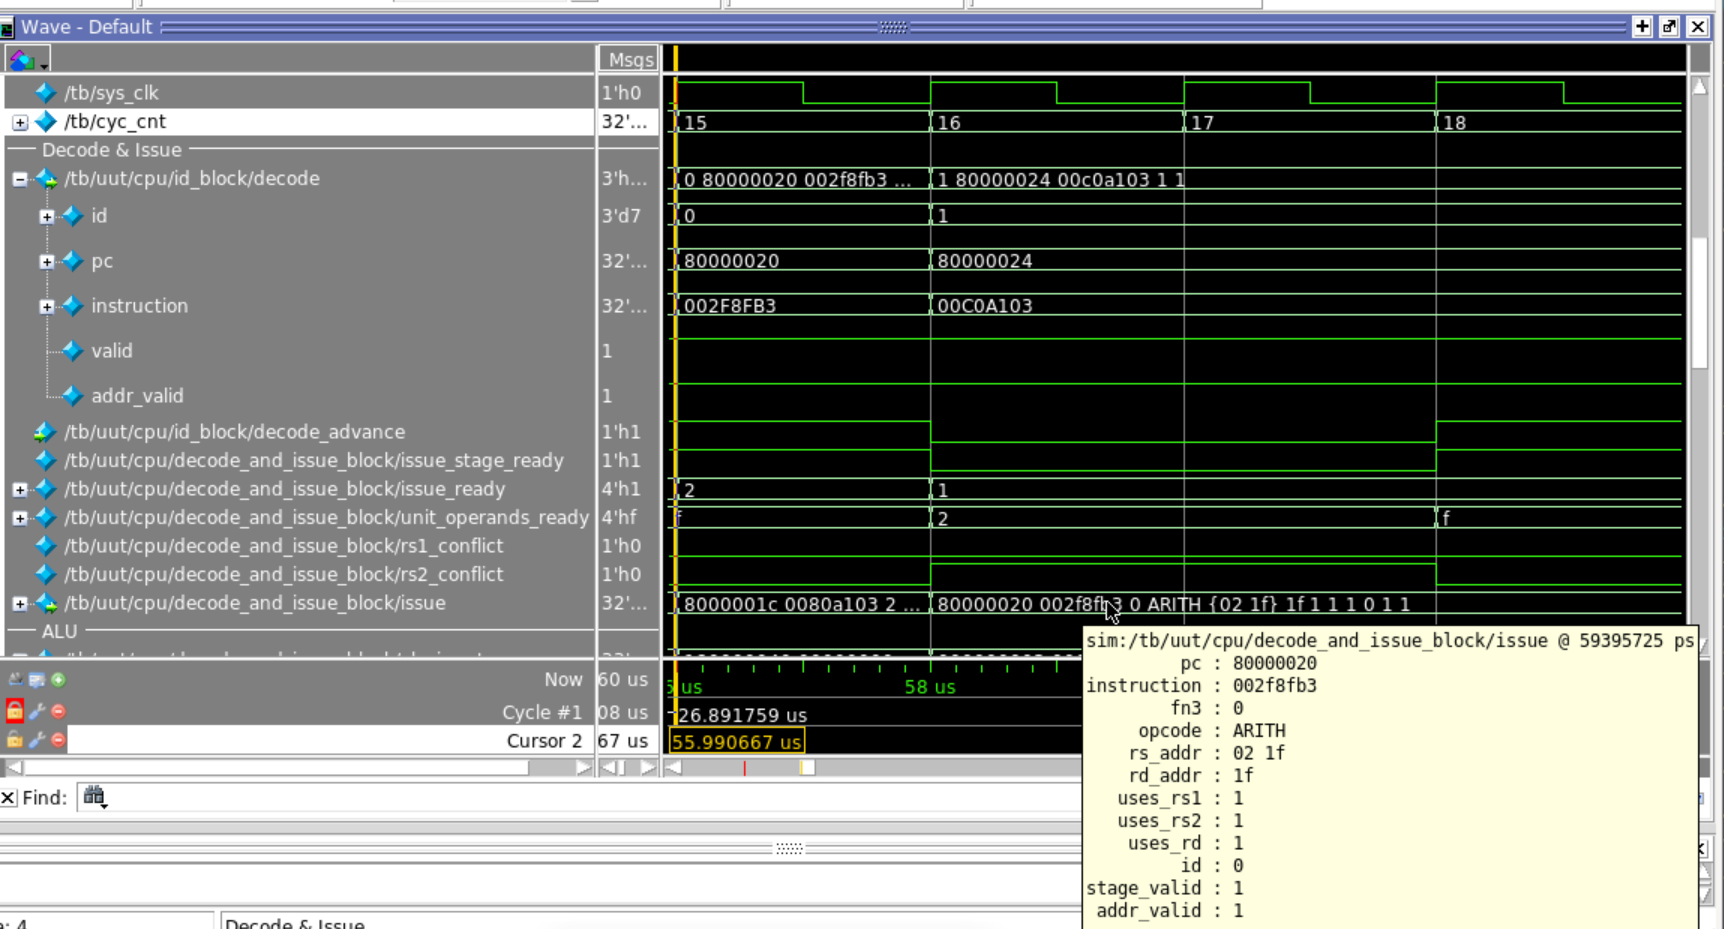
\includegraphics[width=1\textwidth]{images/task3.png}
	\caption{Стадия декодирования и планирования 1-й итерации команды 80000020}
	\label{img:task3}
\end{figure}
\clearpage

Стадия выполнения (ALU) команды 80000008 (согласно варианту) приведена на рисунке~\ref{img:task4}

\begin{figure}[H]
	\centering
	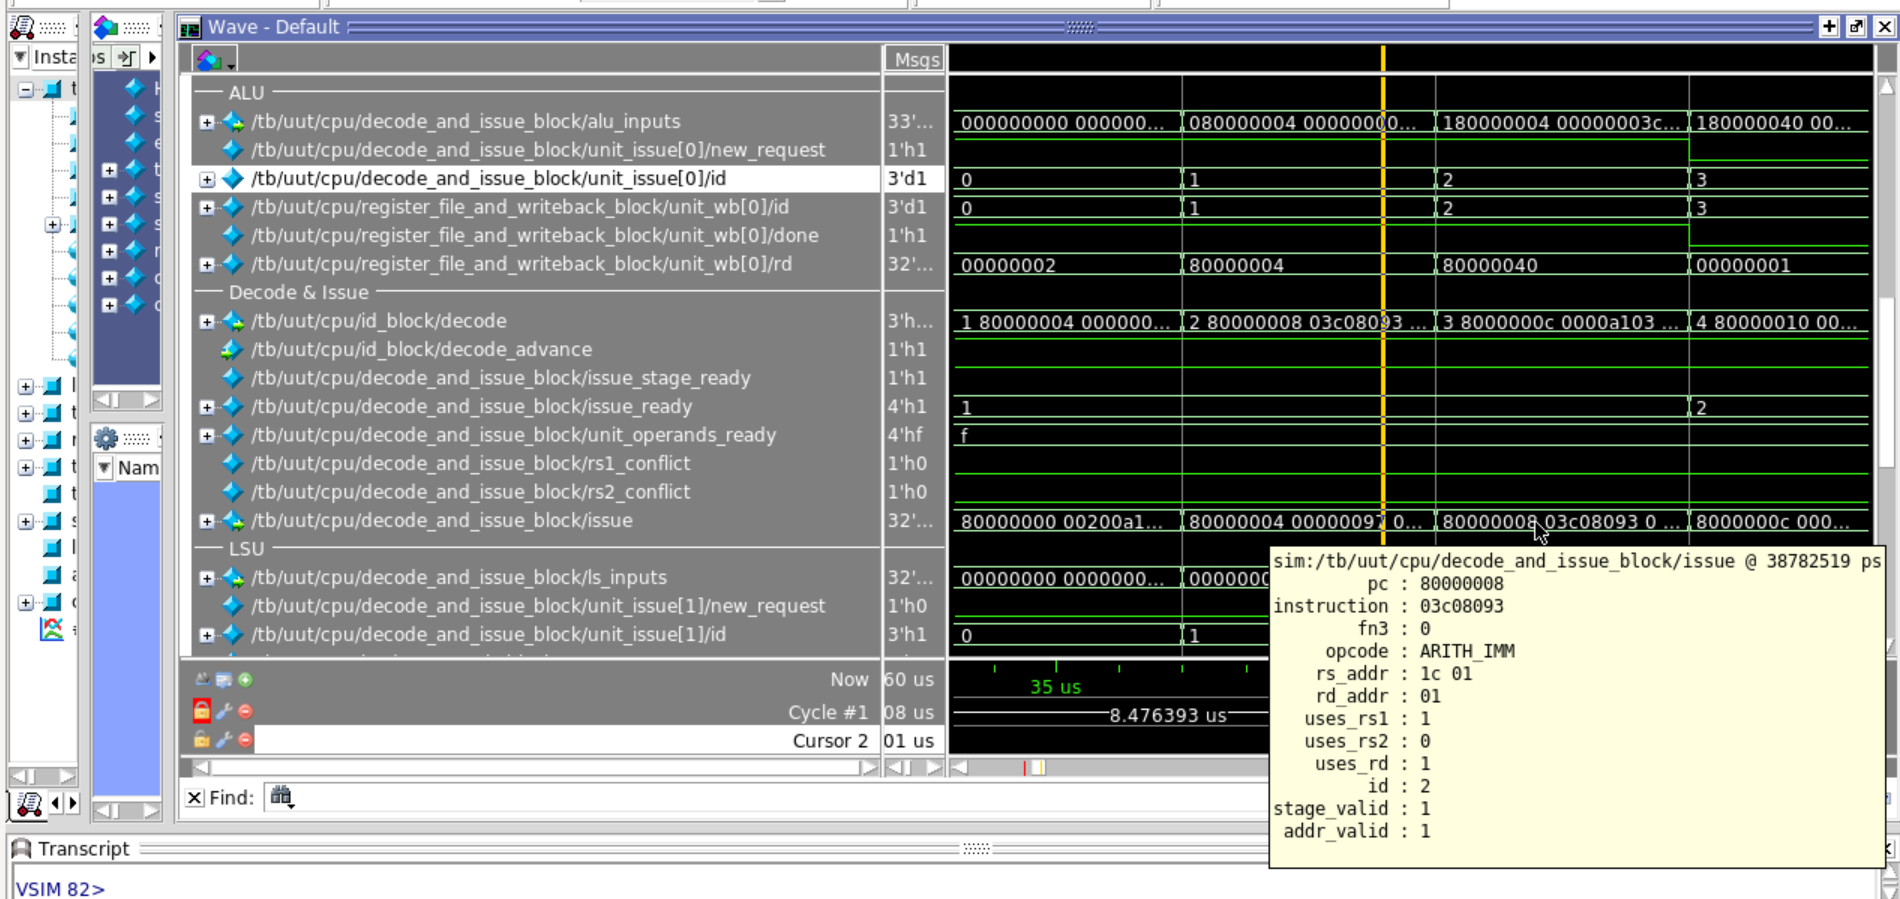
\includegraphics[width=1\textwidth]{images/task4.png}
	\caption{Стадия выполнения команды 80000008}
	\label{img:task4}
\end{figure}
\clearpage

\section{Задания по программе 3-о варианта}

\subsection{Листинг программы}

Исходный текст программы 3-о варианта приведен в листинге~\ref{lst:var3:src}

\lstinputlisting[label=lst:var3:src,caption=Исходный код программы по варианту, captionpos=b]{listings/var3.s}

Листинг программы 3-о варианта, полученный через makefile, приведен в листинге~\ref{lst:var3:lst}

\lstinputlisting[label=lst:var3:lst,caption=Листинг программы по варианту полученный через makefile, captionpos=b]{listings/var3.lst}

16-ричный набор команд программы 3-о варианта приведен в листинге~\ref{lst:var3:hex}

\lstinputlisting[label=lst:var3:hex,caption=Команды программы по варианту в 16-ричном формате, captionpos=b]{listings/var3.hex}

Псевдокод поясняющий работу программы 3-о варианта приведен в листинге~\ref{lst:var3:pseudo}

\lstinputlisting[label=lst:var3:pseudo,caption=Псевдокод к программе по варианту, captionpos=b]{pseudo/pseudo_var3.txt}
\clearpage

\subsection{Стадии выполнения выделенной команды}

В исходном файле выделена команда \textit{add x31, x31, x2}, имеющая адрес $80000014$

Стадии выборки, диспетчеризации (fetch\&dispatch, или F+ID) команды по варианту приведена на рисунке~\ref{img:taskvar_F+ID}

\begin{figure}[H]
	\centering
	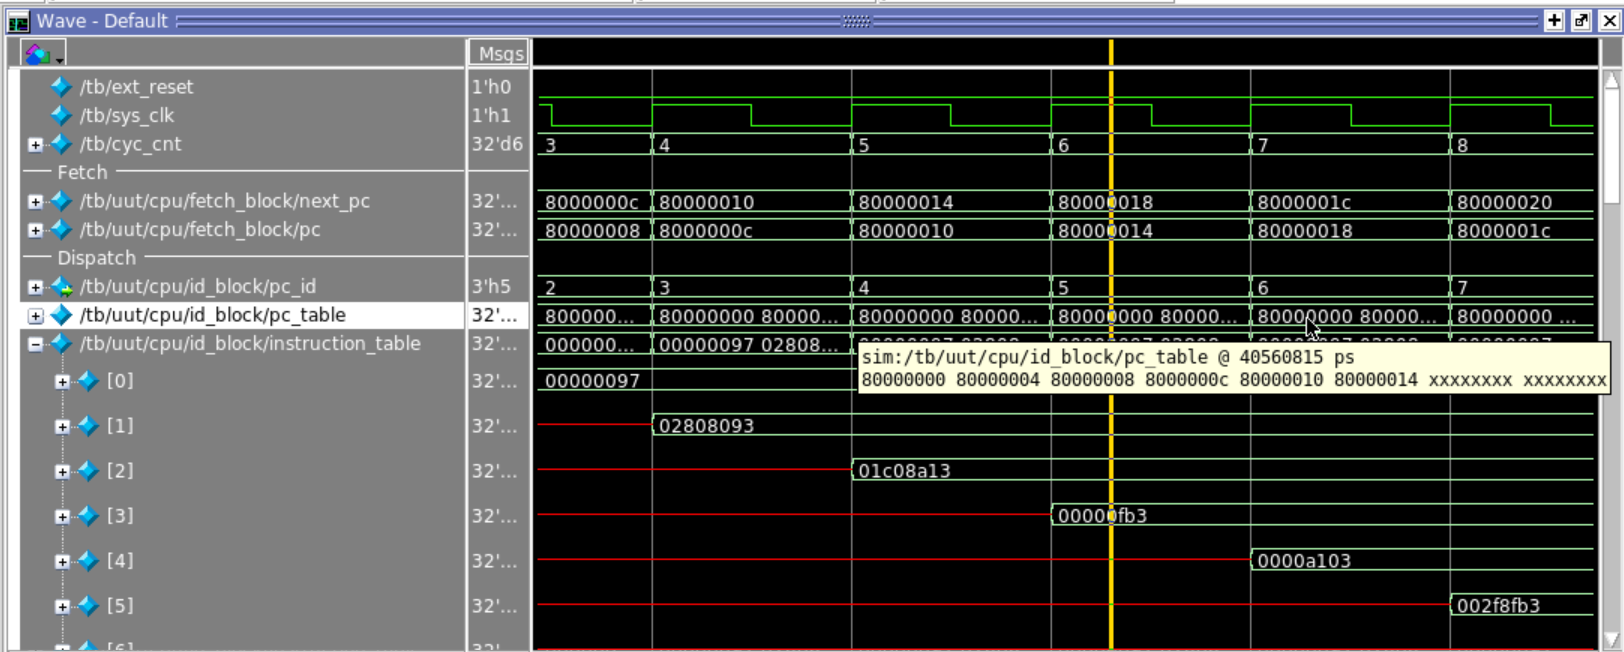
\includegraphics[width=1\textwidth]{images/taskvar_F+ID.png}
	\caption{Стадии выборки и диспетчеризации команды 80000014}
	\label{img:taskvar_F+ID}
\end{figure}

Стадии декодирования и планирования, выполнения (decode\_and\_issue\&ALU, или D+ALU) команды по варианту приведена на рисунке~\ref{img:taskvar_D+CC+ALU}

\begin{figure}[H]
	\centering
	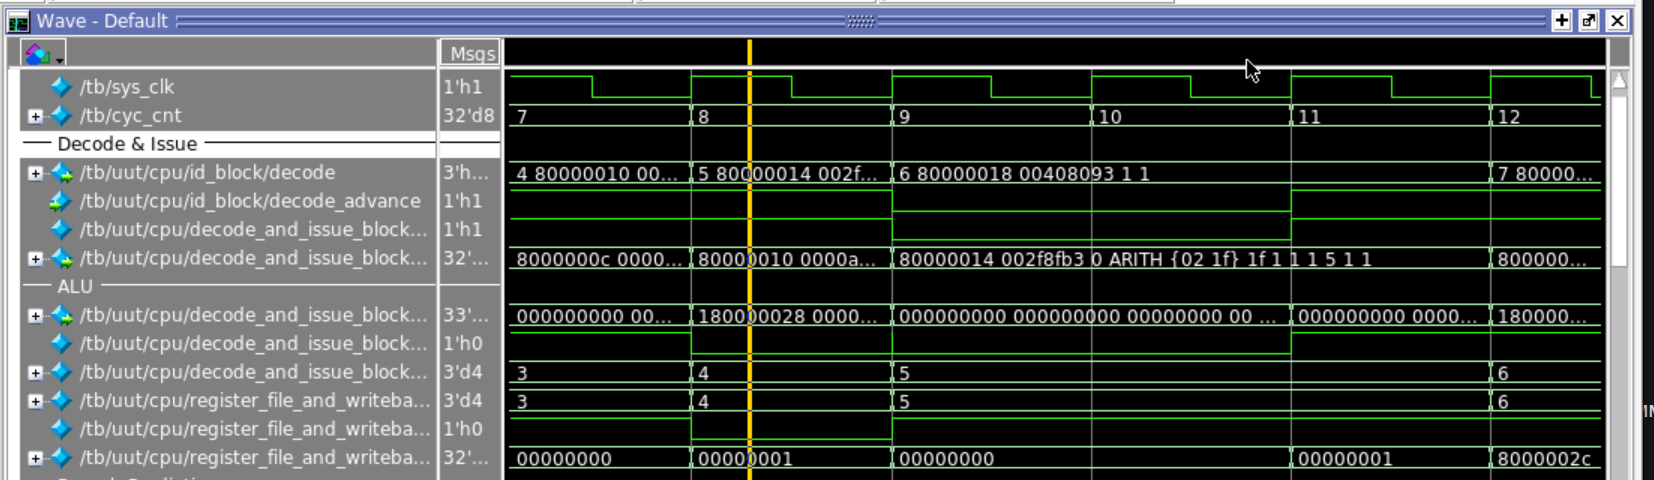
\includegraphics[width=1\textwidth]{images/taskvar_D+CC+AL.png}
	\caption{Стадия декодирования и планирования команды 80000014}
	\label{img:taskvar_D+CC+ALU}
\end{figure}
\clearpage

\subsection{Трасса выполнения программы}

Трасса выполнения программы по варианту приведена на рисунке~\ref{img:var3_trace}

\begin{figure}[H]
	\centering
	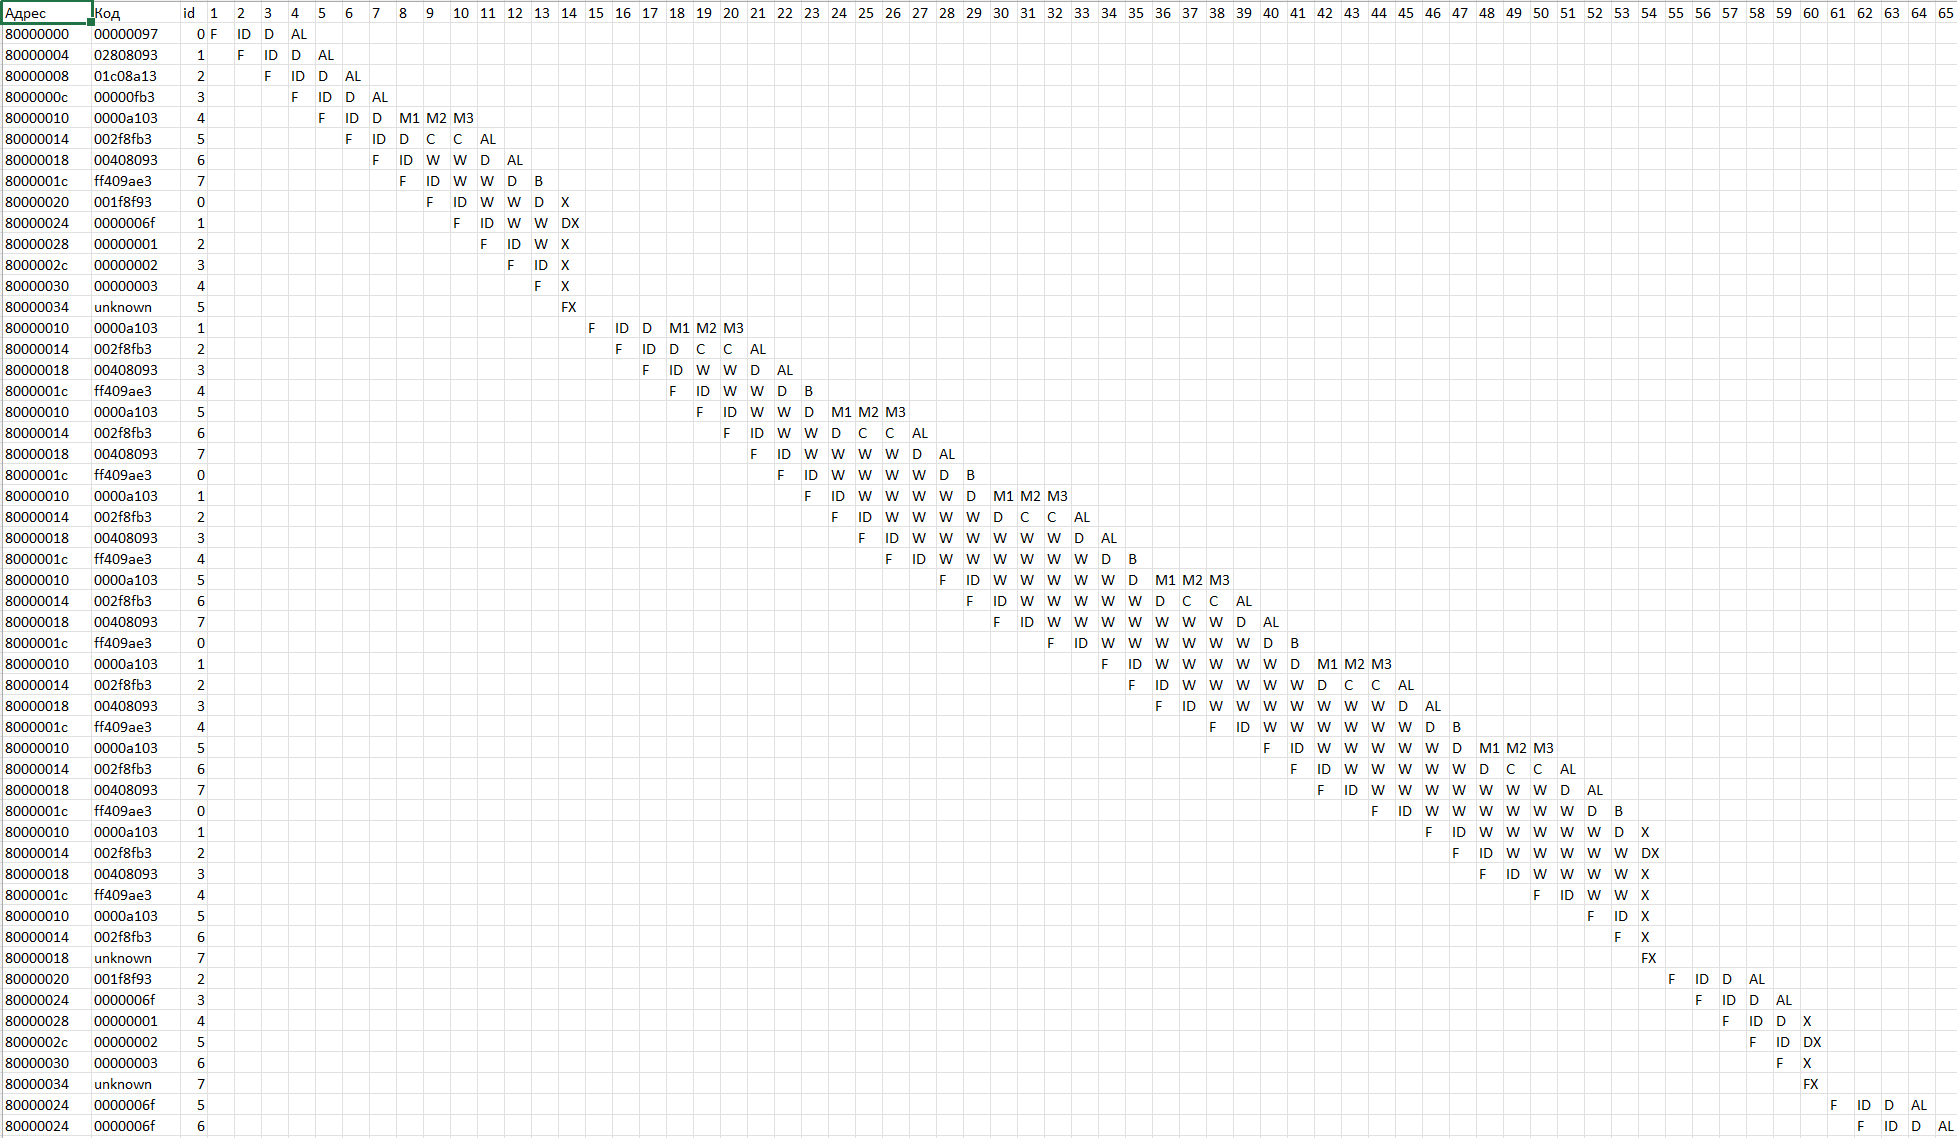
\includegraphics[width=1\textwidth]{images/var3_trace.png}
	\caption{Трасса выполнения программы по варианту}
	\label{img:var3_trace}
\end{figure}

\subsection{Анализ программы}

В трассе выполнения~\ref{img:var3_trace} видно, что арифметическая команда $80000014$, зависящая от результата работы команды чтения из памяти $80000010$, ожидает 2 такта из-за конфликта по регистру (C), в то время как идущая следом за ней $80000018$ выполняет арифметическую операцию с другой переменной. Следовательно, порядок выполнения команд $80000014$ и $80000018$ можно поменять для уменьшения задержки выполнения первой на 1 такт. Для устранения оставшегося такта ожидания имеет смысл добавить один такт простоя командой NOP между командами $80000010$ и $80000014$, чтобы полностью исключить возникновение задержек.
\clearpage

\section{Оптимизация программы по варианту}

\subsection{Листинг программы}

Исходный текст оптимизированной программы 3-о варианта приведен в листинге~\ref{lst:newVar3:src}

\lstinputlisting[label=lst:newVar3:src,caption=Исходный код оптимизированной программы, captionpos=b]{listings/newVar3.s}
\clearpage

Листинг оптимизированной программы 3-о варианта, полученный через makefile, приведен в листинге~\ref{lst:newVar3:lst}

\lstinputlisting[label=lst:newVar3:lst,caption=Листинг оптимизированной программы полученный через makefile, captionpos=b]{listings/newVar3.lst}

16-ричный набор команд оптимизированной программы 3-о варианта приведен в листинге~\ref{lst:newVar3:hex}

\lstinputlisting[label=lst:newVar3:hex,caption=Команды оптимизированной программы в 16-ричном формате, captionpos=b]{listings/newVar3.hex}
\clearpage

\subsection{Трасса оптимизированной программы}

Трасса выполнения оптимизированной программы приведена на рисунке~\ref{img:newVar3_trace}

\begin{figure}[H]
	\centering
	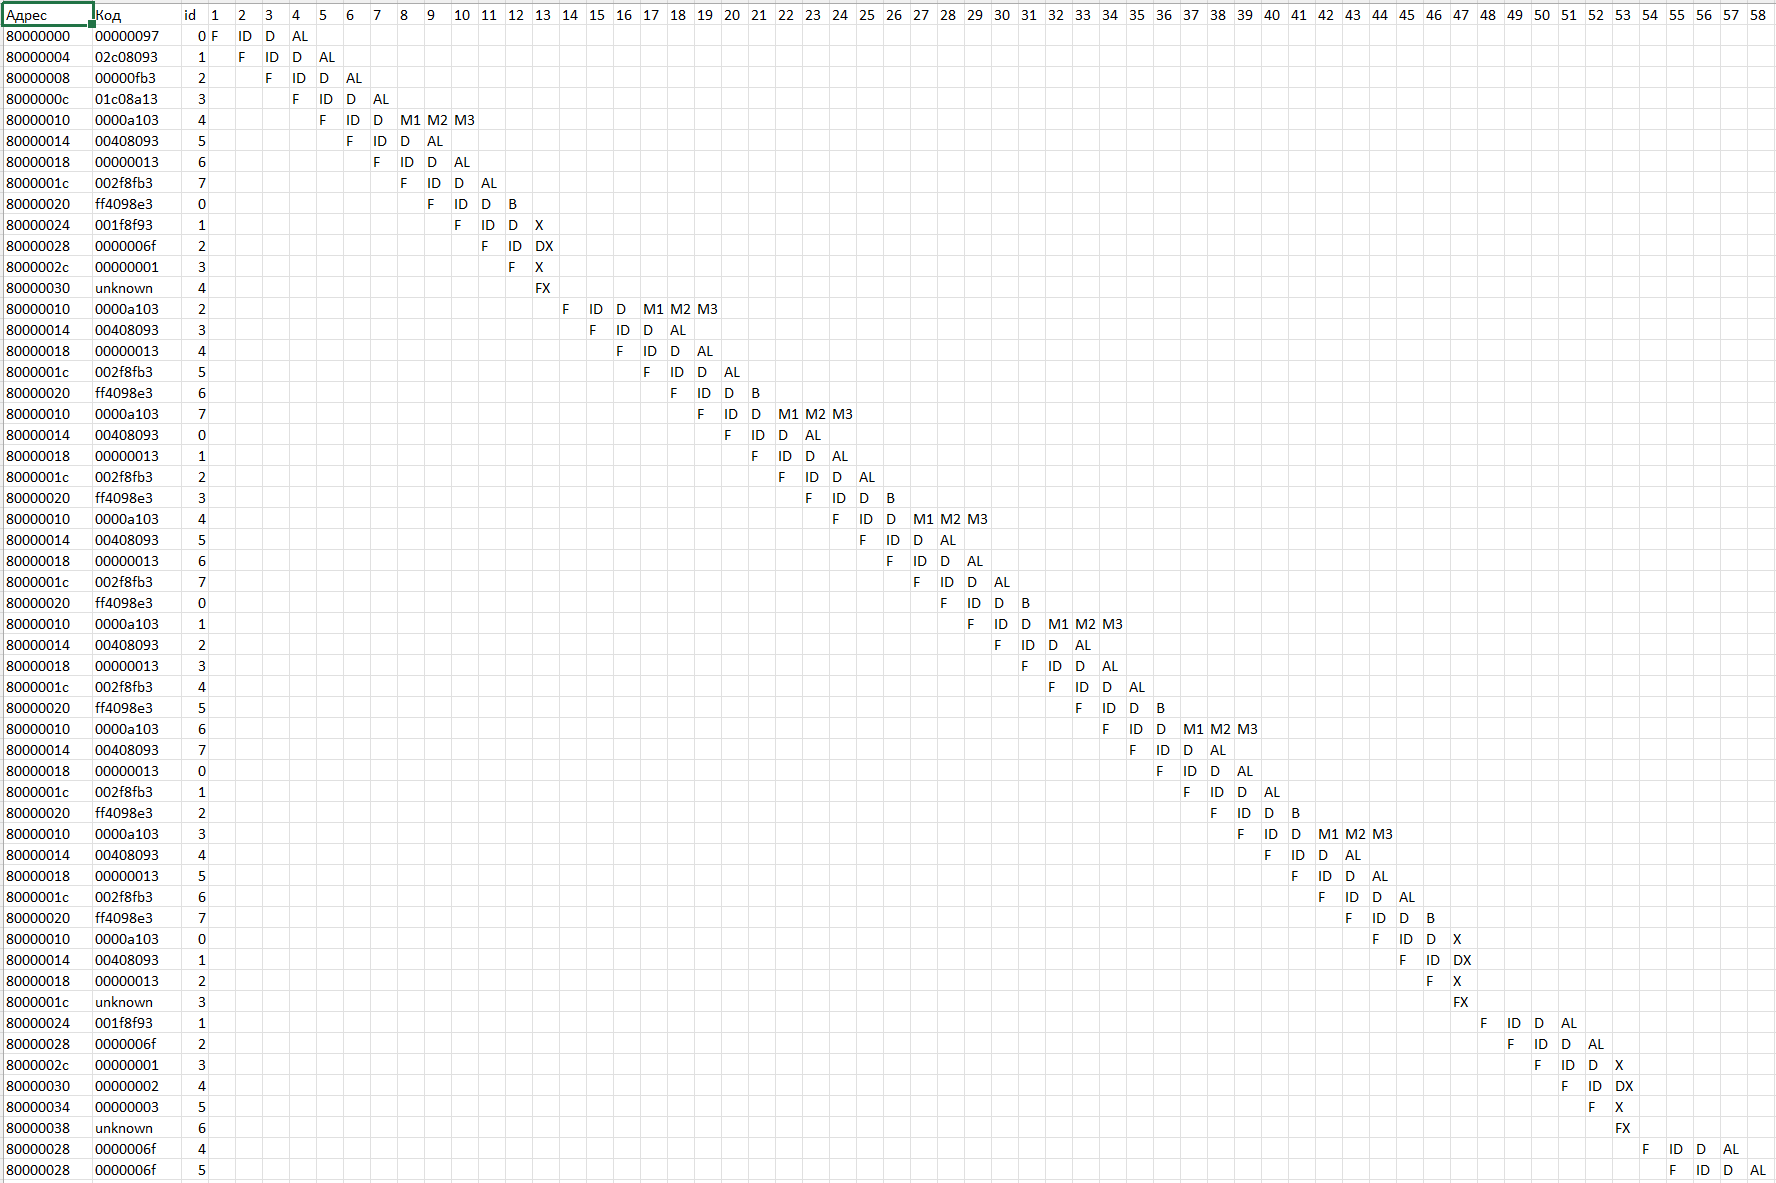
\includegraphics[width=1\textwidth]{images/newVar3_trace.png}
	\caption{Трасса выполнения программы по варианту}
	\label{img:newVar3_trace}
\end{figure}

\section{Вывод}

В результате замены порядка арифметических команд и добавления одного такта ожидания через NOP, время выполнения значимой части кода (идущей до вечного цикла) уменьшилось с 54 тактов до 47, т.е. на $13$\%, а также была полностью устранена нарастающая задержка.

\clearpage
